\chapter{Parameter and table choice}
\label{ch:param}
For the Time-Memory trade-off attack to viable, the right set of
parameters and the right table choice is of huge importance. In this
attack we would ideally want to perform the online phase of the  attack on a modern
high-end laptop/desktop machine. For this to be possible, the right
trade-off between time and memory is needed. For an attack on the
cipher with \code{64-bit} key size, we know a large table is required. But if
we want to make it possible to perform the attack on a (heavily
upgraded) consumer
machine, we need to set an upper bound for the maximal memory
usage. In our attack we set an upper bound of memory usage to around
\code{8TB} of tables[TODO cite to HDD sizes]. We see this as a possible amount of storage if a
consumer machine with a TMTO-attack in mind was to be build.

Knowing this and taking the theory behind the
TMTO-attack\footnote{Chapter \ref{ch:tmto}} into consideration, we
have to argue that this upper bound is required to be hit. For every
trade-off we take towards lower memory usage, the online phase of the
attacks will take a hit.

Another thing to take into consideration when analyzing the parameter
choice and time consumption of the different phases is the table lookup
time. Since generated TMTO tables for a \code{64-bit} key size will
always be larger than a given built machines amount of RAM, look-ups are
done directly on a HDD or SSD. Estimates of how much time is required
for each lookup in a table is hard to do, but will be further analyzed
later in the thesis.

As for success probability of the
the different attacks, we went with $P = 73\%$ as an acceptable
success rate.
We witnessed that for a probability of above $73\%$ the increase,
in both pre-computational cost and the time of the online phase, would
make our initial idea of running the attack on a consumer made PC
unfeasible.

In the following sections we will go through our computations of
parameters for the different TMTO-attacks with these limits set.

\section{Hellman Table}
All calculations of parameters follows the theory provided in
\ref{sec:hmtheory}.

Concidering the theory and above mentioned formulas, a approximation of the best parameters for a $73\%$ success rate table can be made.
As stated earlier the memory requirements will meet the upper bound of
\code{8TB}.
As the success probability already is set we can find the respective parameters and compare them.

\begin{figure}[H]
  \centering
  \begin{minipage}{0.45\textwidth}
    \centering
    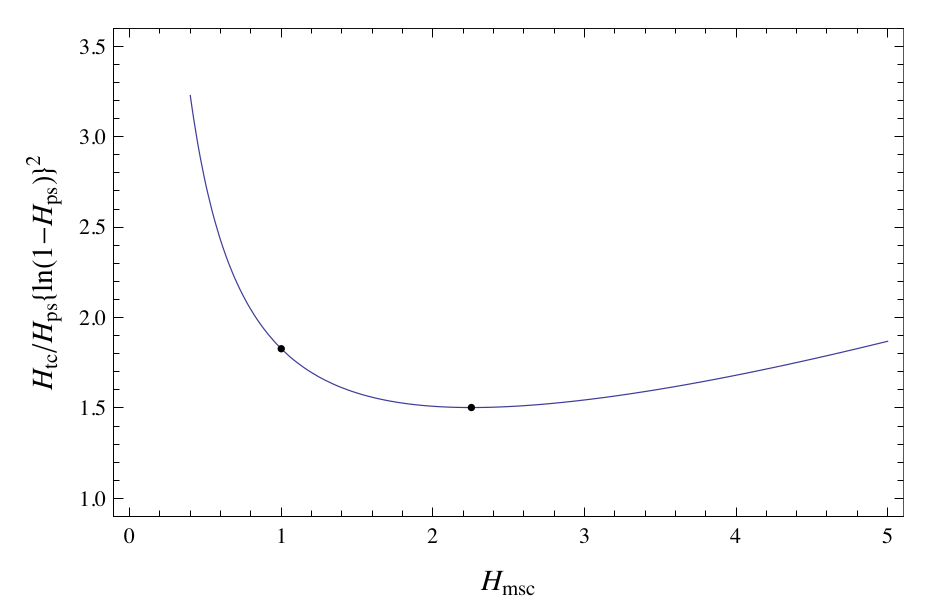
\includegraphics[width=1.2\textwidth]{figures/HellmanTradeOff.png}
    \captionof{figure}{Figure from \cite{176}}
    \label{fig:hellTC}
  \end{minipage}\hfill
  \begin{minipage}{0.45\textwidth}
    \centering
    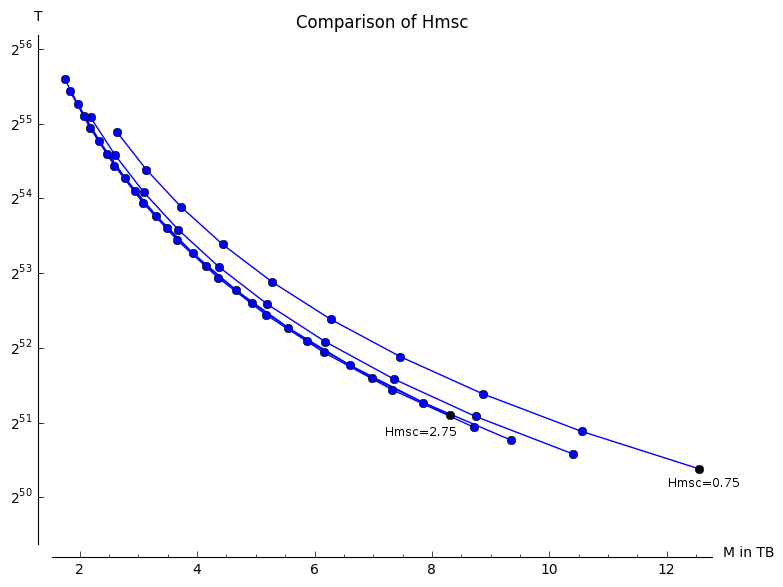
\includegraphics[width=1.2\textwidth]{figures/compareHmsc.png}
    \captionof{figure}{$H_{msc}$ from 0.75 to 2.75}
    \label{fig:hellHmsc}
  \end{minipage}
\end{figure}
As we know from \cite{176} a lower trade-off coefficient results in a
better trade-off. Figure \ref{fig:hellHmsc} shows a graph of the
trade-off coefficient for a set success rate and $H_{msc}$.
As seen on \ref{fig:hellTC} the best possible trade-off is achieved
when $H_{msc}$ is between 1 and 2.25. This is further shown in
\ref{fig:hellHmsc} where, as $H_{msc}$ grows, the smaller the memory
required for the tables get. This effect decreases as $H_{msc}$ grows
larger than 2.25. A side effect of an increasing $H_{msc}$ is it's
influence on the pre-computational cost and the efficiency of the
trade-off. The optimal value of $H_{msc}$ is when the trade-off
efficiency is lowest. An $H_{msc}$ set to $2.25$ makes for the most
efficient trade-off.

Table \ref{tab:hellparam} shows a generated table of Hellman
parameters for $H_{msc} =2.25$.
\begin{table}[H]
  \centering
  \text{\texttt{Success{ }={ }0.73,{ }Hmsc{ }={ }2.25,{ }Hcr{ }={ }0.74,{ }Htc{ }={ }1.88{ }Hpc{ }={ }1.77} }
\begin{tabular}{lllll}
m & t & l & M in TB & T \\\hline
$2^{12.00}$ & $2^{26.58}$ & $2^{26.24}$ & $5.18$ & $2^{52.44}$ \\
$2^{12.20}$ & $2^{26.48}$ & $2^{26.14}$ & $5.55$ & $2^{52.24}$ \\
$2^{12.40}$ & $2^{26.38}$ & $2^{26.04}$ & $5.95$ & $2^{52.04}$ \\
$2^{12.60}$ & $2^{26.28}$ & $2^{25.94}$ & $6.38$ & $2^{51.84}$ \\
$2^{12.80}$ & $2^{26.18}$ & $2^{25.84}$ & $6.84$ & $2^{51.64}$ \\
$2^{13.00}$ & $2^{26.08}$ & $2^{25.74}$ & $7.33$ & $2^{51.44}$ \\
$2^{13.20}$ & $2^{25.98}$ & $2^{25.64}$ & $7.85$ & $2^{51.24}$ \\
$2^{13.40}$ & $2^{25.88}$ & $2^{25.54}$ & $8.42$ & $2^{51.04}$ \\
$2^{13.60}$ & $2^{25.78}$ & $2^{25.44}$ & $9.02$ & $2^{50.84}$ \\
$2^{13.80}$ & $2^{25.68}$ & $2^{25.34}$ & $9.67$ & $2^{50.64}$ \\
\end{tabular}
  \caption{Hellman Parameters}
  \label{tab:hellparam}
\end{table}
We can now select the parameters we want our Attack to use, As Hmsc has been optimized we selected : $m=2^{13.2}$, $t=2^{25.98}$ and $l=2^{25.64}$.
This gives us a table of size \code{7.85 TB}.
\section{Distinguished Points Table}
For this section we assume that $\hat{t}$ is sufficiently large.

All calculations of parameters follow the theory provided in
\ref{sec:dptheory}.

Again we use the set upper bound for the memory and the success ratio.
As shown in \ref{fig:dpHmsc} the smaller the matrix stopping constant
gets the larger the table gets. The time memory coefficient is most
efficient at 0.56 \cite{176} the paper also states that a $D_{msc}$ above
0.56 should be avoided. Therefore the matrix stopping constant has been
set to 0.56, using the formulas for optimal parameters from \cite{176}
\ref{tab:DPparam} is generated.(note chain length is the approximated average chain length)
\begin{figure}[H]
  \centering
  need to put lables on the elements from left to right 0.2, 0.3, 0.56, 0.75, 1.00, 1.25
    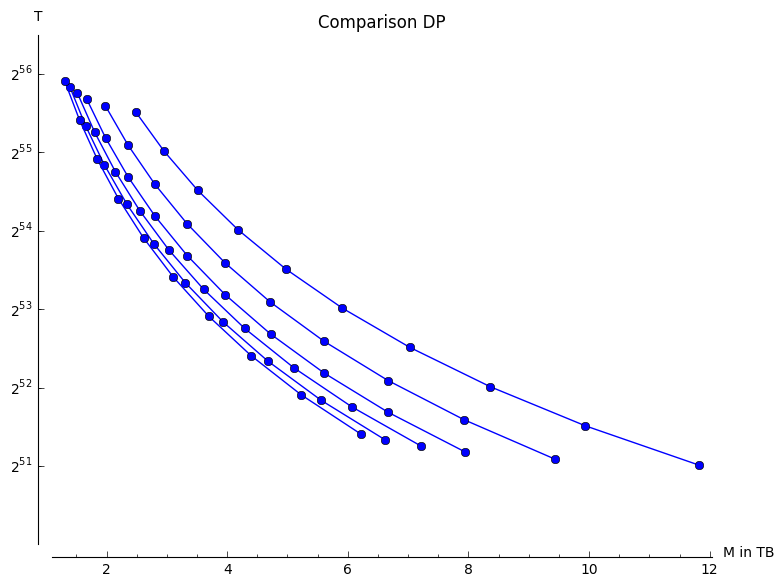
\includegraphics[width=0.5\textwidth]{figures/compareDmsc.png}
    \captionof{figure}{$D_{msc}$ from 0.2 to 1}
    \label{fig:dpHmsc}
\end{figure}
\begin{table}[H]
  \centering
  \text{\texttt{Success{ }={ }0.73,{ }Dmsc{ }={ }0.56,{ }Dcr{ }={ }0.81,{ }Dtc{ }={ }8.77{ }Dpc{ }={ }1.60} }
\begin{tabular}{lllll}
m & t & l & M in TB & T \\\hline
$2^{12.00}$ & $2^{25.58}$ & $2^{27.10}$ & $4.72$ & $2^{52.69}$ \\
$2^{12.20}$ & $2^{25.48}$ & $2^{27.00}$ & $5.06$ & $2^{52.49}$ \\
$2^{12.40}$ & $2^{25.38}$ & $2^{26.90}$ & $5.42$ & $2^{52.29}$ \\
$2^{12.60}$ & $2^{25.28}$ & $2^{26.80}$ & $5.81$ & $2^{52.09}$ \\
$2^{12.80}$ & $2^{25.18}$ & $2^{26.70}$ & $6.23$ & $2^{51.89}$ \\
$2^{13.00}$ & $2^{25.08}$ & $2^{26.60}$ & $6.67$ & $2^{51.69}$ \\
$2^{13.20}$ & $2^{24.98}$ & $2^{26.50}$ & $7.15$ & $2^{51.49}$ \\
$2^{13.40}$ & $2^{24.88}$ & $2^{26.40}$ & $7.67$ & $2^{51.29}$ \\
$2^{13.60}$ & $2^{24.78}$ & $2^{26.30}$ & $8.22$ & $2^{51.09}$ \\
$2^{13.80}$ & $2^{24.68}$ & $2^{26.20}$ & $8.81$ & $2^{50.89}$ \\
\end{tabular}
  \caption{DP Parameters}
  \label{tab:DPparam}
\end{table}
This leaves us to select our parameters in this case we have optimized the Dmsc, we could discuss lowering it to lower the precomputational cost but we go with the parameters: $m=2^{13.40}$  $t=2^{24.88}$  $l=2^{26.40}$.
This gives us a table that is \code{7.67 TB}.
\section{Rainbow Table}
\label{sec:rainbowparam}
For the Rainbow Table TMTO attack, we again set \code{8TB} as the
upper bound for memory consumption.

All calculations of parameters follows the theory provided in
\ref{sec:raintheory}.

Conveniently \cite[Fig.4]{176} shows that with our chosen success rate
$P$ the trade-off effiency is actually lowest when the table count is
set to 1.

In our calculations, we assume a sequential approach is done in the
pre-computational phase. This allows us to remove half of the memory,
as only the end point needs to be stored.

As we have a chosen success rate $P$ set, \cite[Proposition
29]{176} shows that from a given $P$ we can calculate a lower bound
for $R_{msc}$ as follows
\[R_{ps} = 1 - \left( \frac{2}{2 + R_{msc}}^{2l} \right) \Rightarrow R_{msc} = 2 ((1 - R_{ps})^{-\frac{1}{2l}} - 1)\]
Where $R_{ps}$ is the success probability of a rainbow attack. With
that in mind we can now for different values of $m$ compute the
corresponding $t$ value where the $R_{msc}$ is satisfied.

Table \ref{tab:rainparam} shows the relation between \code{t} and
\code{m} in a Rainbow attack, when the success rate of $73\%$ is set\footnote{Tables for $P = 58\%, P = 73\%, P = 90\%$ and tables $l=1..3$ are generated and can be
found in Appendix \ref{sec:rainbowtab}.}. Figures \ref{fig:param73}
and \ref{fig:time73} shows the graphical representation of the table.

\begin{table}[H]
  \centering
  \text{\texttt{Success{ }={ }0.730000,{ }Rmsc{ }={ }1.849002,{ }l{ }={ }1,{ }Offline{ }phase{ }={ }2{\char`\^}64.886747}}
  \begin{tabular}{llll}
    m & t & M(TB) & T \\ \hline
    $2^{35.50}$ & $2^{29.39}$ & $0.39$ & $2^{56.58}$ \\
    $2^{36.00}$ & $2^{28.89}$ & $0.55$ & $2^{55.58}$ \\
    $2^{36.50}$ & $2^{28.39}$ & $0.78$ & $2^{54.58}$ \\
    $2^{37.00}$ & $2^{27.89}$ & $1.10$ & $2^{53.58}$ \\
    $2^{37.50}$ & $2^{27.39}$ & $1.55$ & $2^{52.58}$ \\
    $2^{38.00}$ & $2^{26.89}$ & $2.20$ & $2^{51.58}$ \\
    $2^{38.50}$ & $2^{26.39}$ & $3.11$ & $2^{50.58}$ \\
    $2^{39.00}$ & $2^{25.89}$ & $4.40$ & $2^{49.58}$ \\
    $2^{39.50}$ & $2^{25.39}$ & $6.22$ & $2^{48.58}$ \\
    $2^{39.80}$ & $2^{25.08}$ & $7.65$ & $2^{47.98}$ \\
    $2^{40.00}$ & $2^{24.89}$ & $8.80$ & $2^{47.58}$ \\
  \end{tabular}
  \caption{Rainbow Parameters}
  \label{tab:rainparam}
\end{table}
\begin{figure}[H]
  \centering
  \begin{minipage}{.5\textwidth}
    \centering
    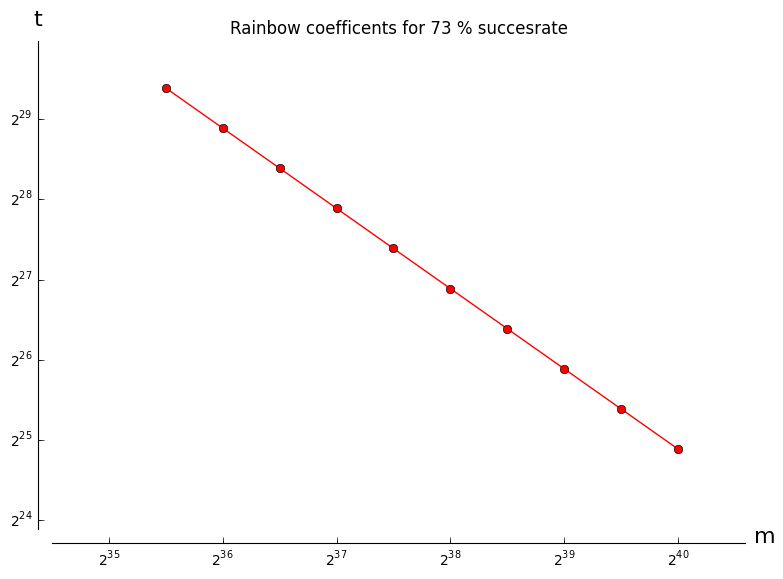
\includegraphics[scale=0.3]{figures/RainbowCoef73.png}
    \captionof{figure}{Rainbow Parameters 73\% success}
    \label{fig:param73}
  \end{minipage}%
  \begin{minipage}{.5\textwidth}
    \centering
    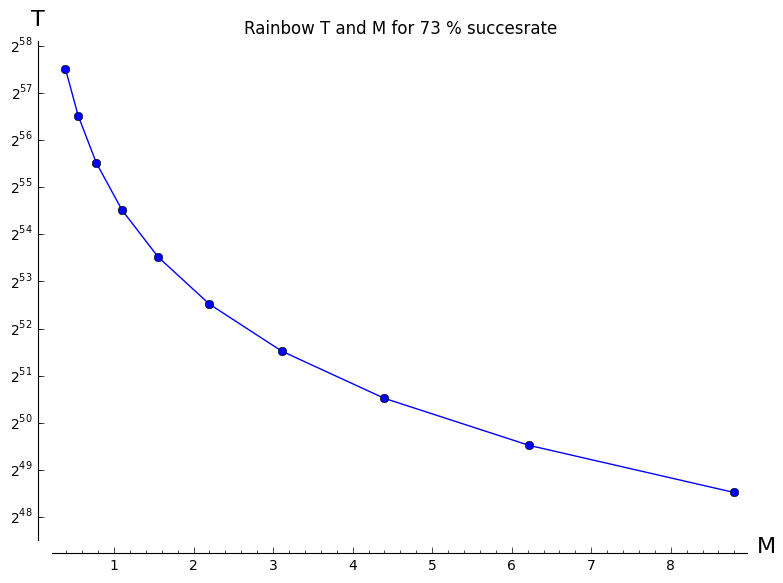
\includegraphics[scale=0.3]{figures/RainbowTime73.png}
    \captionof{figure}{Rainbow TMTO 73\% success}
    \label{fig:time73}
  \end{minipage}
\end{figure}
Looking at table \ref{tab:rainparam} and figures \ref{fig:param73}
and \ref{fig:time73}\footnote{See Appendix \ref{sec:rainbowgraphs} for
  full size graphs} we select the parameters for our attack. As the
trade-off at 73$\%$ is most efficient with one table $l=1$ as for m
and t we decided to use $m=2^{39.8}$ and $t=2^{25.08}$. This leaves us
with $M = 2^{45.79} = 7.65$TB and $T = 2^{48.98}$ 

\newpage
\section{Comparison and choice of table}
Three different attacks have been described and explored. The above
tables and graphs provide a range of possible parameters which hold true for our
constraints.

Table \ref{tab:compare} shows our selected parameters for each attack,
the memory cost, the pre-computational time and the online time. 

It can can be seen in the table Hellman and DP trade-off are quite similar in
their parameters. The biggest difference as stated in \ref{sec:dptheory}
is the amount of look ups that are required. Where Hellman
requires $m \cdot l$, the DP attack only need to look through each
table once the distinguished point is reached. When attacks get
larger, and more tables is required the Hellman attack will therefore
scale badly, and the DP attack will be to prefer.

Now to choose between rainbow attack and DP attack. As the rainbow attack
uses less but much larger tables, it is harder to compare $m$, $m$ and
$l$. However we can still compare the pre-computational and online time. The
pre-computational cost is approximately the same for all the attacks,
but the online time for the DP attack (and Hellman) is almost 5 times larger than
the rainbow attack.
\begin{table}[H]
  \centering
  \begin{tabular}{|l|cccccc}
    \hline
    \rowcolor[HTML]{EFEFEF}
    Attack  & \multicolumn{1}{c|}{\cellcolor[HTML]{EFEFEF}m} & \multicolumn{1}{c|}{\cellcolor[HTML]{EFEFEF}t} & \multicolumn{1}{c|}{\cellcolor[HTML]{EFEFEF}l} & \multicolumn{1}{c|}{\cellcolor[HTML]{EFEFEF}M in TB} & \multicolumn{1}{c|}{\cellcolor[HTML]{EFEFEF}Precomp} & \multicolumn{1}{c|}{\cellcolor[HTML]{EFEFEF}Online} \\ \hline
    Hellman & $2^{13.2}$                                     & $2^{25.98}$                                    & $2^{25.64}$                                    & 7.85                                                 & $2^{64.82}$                                          & $2^{51.24}$                                         \\ \cline{1-1}
    \rowcolor[HTML]{EFEFEF}
    DP      & $2^{13.4}$                                     & $2^{24.88}$                                    & $2^{26.4}$                                     & 7.67                                                 & $2^{64.68}$                                          & $2^{51.29}$                                         \\
    Rainbow & $2^{39.8}$                                     & $2^{25.08}$                                    & 1                                              & 7.65                                                 & $2^{64.88}$                                          & $2^{48.98}$                                         \\ \cline{1-1}
  \end{tabular}
  \caption{Comparison of parameter choices}
  \label{tab:compare}
\end{table}

From these tables we can pretty easily see that theoretically the rainbow attack
will be preferable. One thing the tables doesn't take into
account, is the amount of look ups needed in the online phase of the
rainbow attack. We know that $t$ look ups is required, but it is hard
to estimate exactly how much time is required on each look up. The
look ups and their effect on the attack will be tested in chapter \ref{ch:anal}.


%%% Local Variables:
%%% mode: latex
%%% TeX-master: "Thesis"
%%% End:
